\section{Experiments}

For the following experiments, the Sentinel-2 bands of the BigEarthNet-MM dataset \cite{bigEartNetMM} are used. The latent representations of this data are examined intrinsically using UMAP feature visualization to determine if the embeddings naturally group similar items together and separate dissimilar ones. Extrinsic evaluation assesses the model's performance on an external downstream task, which depends on both the foundation model and the adaptation mechanism \cite{foundationModels}. In the performed extrinsic experiments, classifying the BigEarthNet data is chosen as the downstream task. Linear probing and classification with a simple Multiple Layer Perceptron are examined. The model's performance is analysed without retraining it on the classification data to only evaluate the information stored in the feature vectors. \\
The authors of the contrastive learning model \cite{geoAwareSelfSuper} provide their code as well as weights for four models: the original MoCo-v2 model, the MoCo-v2 model additionally trained on the geo-location pre-text task (MoCo-v2+Geo), the MoCo-v2 model trained with temporal positive pairs (MoCo-v2+TP), and the MoCo-v2 model trained on the pretext task in combination with temporal positive pairs (MoCo-v2+Geo+TP). They use the ResNet-50 \cite{resnet} architecture to parameterize the query and key encoders $f_q$ and $f_k$ for each model. For inferencing only the query encoder ist used. The weights are pre-trained on the fMoW \cite{fmow} dataset. The evaluation setup is illustrated in Fig. \ref{fig:setup}.

\subsection{Data - BigEarthNet-MM}

The BigEarthMet-MM benchmark dataset by Sumbul et al. \cite{bigEartNetMM} is designed for multi-modal and multi-label remote sensing applications. It consists of satellite images, i.e.  590,326 pairs of Sentinel-1 and Sentinel-2 image patches, acquired over 10 different European countries, each of which $120\times120$ pixels. The patches are annotated with multi-labels provided by the CORINE Land Cover (CLC) map of 2018, such as \textit{Broad-leaved forest} and \textit{Beaches, dunes, sands}. In total, the image patches are representative of 43 CLC classes. Sumbul et al. \cite{bigEartNetMM} also created a new class-nomenclature by modifying the CLC multi-labels resulting in 19 classes. CLC classes that are not feasible to be identified by only using single-date BigEarthNet-MM images are removed and others are grouped into new classes. \\
For the evaluation of the contrastive learning foundation model, 19 classes were chosen. Since the foundation model is designed to accept inputs of one modality at a time, only the Sentinel-2 images are used (BigEarthNet-S2). Examples are shown in Fig. \ref{fig:BigEarth}. \\
During the self-supervised pretraining of the foundation model, the fMoW data is normalized using z-score normalization. The fMoW images consist of RGB channels, which fit the ResNet-50 architecture designed for data with three input color channels. The spectral bands of the BigEarthNet-S2 dataset also include the visible spectrum bands: Red (B04), Green (B03), and Blue (B02). By selecting these bands and normalizing the data, the BigEarthNet-S2 images are prepared similarly to the fMoW images, providing a solid basis for meaningful inference results.

\subsection{UMAP Feature Visualization}
UMAP (Uniform Manifold Approximation and Projection) is a manifold learning technique for dimensionality reduction by McInnes et al. \cite{umap}. It visualizes high-dimensional data in a low-dimensional space while preserving local and global structures of the data. This makes it particularly useful for visualizing complex datasets such as feature embeddings. The technique is based in Riemannian geometry and algebraic topology. \\
By transforming high-dimensional data into a 2D or 3D space, UMAP allows for the visualization of the distribution of embeddings. Given that the BigEarthNet-S2 dataset provides multi-class labels, this technique makes it possible to observe if embeddings of images within the same class cluster together, indicating low distances between them. Since images of the same class share many similar features, their embeddings should ideally be close to each other. \\
The embedding layer of the contrastive learning models is the final layer, allowing the outputs of the inferencing to be directly interpreted as latent feature representations. The feature vectors extracted by the provided models have a size of 128. For the visual evaluation these vectors are transformed into a 2D space. \\
Results for the categories \textit{arable land}, \textit{coniferous forest} and \textit{marine waters} are shown in Fig. \ref{fig:umap}. Feature vectors from the BigEarthNet-S2 test dataset are used here. In all four models, data points belonging to the \textit{marine waters} category (blue) form a distinct cluster, significantly separated from other points (grey). For most other categories, such as \textit{arable land} and \textit{coniferous forest}, there are only minor distribution shifts between the points of a given category and the other data points. These observations are consistent across all four models. Detailed UMAP visualizations, separated by each of the 19 classes, can be found in the supplementary material. This visual evaluation does not reveal performance differences between the four contrastive learning models. However, the test demonstrates that the feature embeddings retain some semantic information from the input images.

\subsection{Classification Downstream Task}
\label{sec:classification}
%In this section, the foundation models' performance is evaluated based on their ability to complete the BigEarthNet-S2 multi-label classification downstream tasks. 
Most of the existing deep learning based methods assume that training images are annotated by single-labels, however remote sensing images typically contain multiple classes and thus
can simultaneously be associated with multi-labels \cite{benchmark}. The following tests intent to show how well the models' learned representations can be transferred and utilized in such a real-world remote sensing scenario: the BigEarthNet-S2 multi-label classification tasks.

\begin{table*}[h]
\centering
\begin{tabular}{c|cccc|cccc|c}
& \multicolumn{4}{|c|}{\textbf{Linear probing}} & \multicolumn{4}{|c|}{\textbf{MLP}} & \textbf{Baseline} \\
& MoCo-v2 & +Geo & +TP & +Geo+TP & MoCo-v2 & +Geo & +TP & +Geo+TP & K-Branch CNN \\ \hline
$R_{macr}$ & 0.239 & \textbf{0.241} & \textbf{0.241} & 0.224 & 0.394 & \textbf{0.417} & 0.395 & 0.382 & \textit{\textbf{0.468}} \\
$F^2_{macr}$ & 0.260 & \textbf{0.267} & 0.265 & 0.245 & 0.424 & \textbf{0.448} & 0.426 & 0.413 & \textit{\textbf{0.446}} \\
$F^2_{micr}$ & \textbf{0.381} & 0.360 & 0.367 & 0.349 & 0.555 & \textbf{0.570} & 0.546 & 0.538 & \textit{\textbf{0.610}} \\
$HL$ & \textbf{0.115} & 0.117 & \textbf{0.115} & 0.119 & 0.091 & \textbf{0.090} & 0.093 & 0.095 & \textit{\textbf{0.041}} \\
$OE$ & \textbf{0.311}& 0.344 & 0.327 & 0.363 & 0.177 & \textbf{0.175} & 0.181 & 0.194 & \textit{\textbf{0.063}} \\
\end{tabular}
\caption{Multi-label classification results of the experiments in section \ref{sec:classification}. The linear probing and MLP classifiers are trained on the foundation models' embedding outputs for the 19-class BigEarthNet-S2 task, while the baseline model results pertain to the 43-class task.}
\label{tab:classification}
\end{table*}

\subsubsection{Performance Metrics}
To evaluate any multi-label classification approach it is necessary to analyse more than only the number of correct predictions. Therefore, several performance metrics are used to present the results of the multi-label experiments: Recall (R), F2-Score (F2), Hamming loss (HL) and One error (OE).  \\
There are different ways to calculate the classification based metrics recall and F2-Score. Macro averaging gives equal importance to each class by first computing the metrics per class and then averaging the class results. Micro averaging computes the metrics globally by treating each individual prediction as an atomic unit. \cite{benchmark} \\
During the experiments of these sections the recall is calculated with macro averaging and for the F2-Score both, micro and macro averaging, are reported. The following calculatioins originate from Sumbul et al. \cite{benchmark}. \\
Let $TP_{ij}$, $FP_{ij}$, $FN_{ij}$ and $FP_{ij}$ indicate the conditions of true positive, false positive, false negative and true negative for the $i^{th}$ sample and $j^{th}$ class label ($l_j$), where exactly one is true, value $1$, and the other three take $0$. The recall with macro averaging is expressed as follows: 
\begin{equation}
    R_{macr}=\frac{1}{S}\sum_{j=1}^S \frac{\sum_{i=1}^M TP_{ij}}{\sum_{i=1}^M TP_{ij}+FN_{ij}},
\end{equation}
where $S$ is the number of classes and $M$ the number of samples. The F2-Score is the weighted harmonic mean of the metrics precison and recall. It is defined as follows:
\begin{equation}
    F_{macr}^2 = \frac{1}{S}\sum_{j=1}^S \frac{\sum_{i=1}^M 5TP_{ij}}{\sum_{i=1}^M 5TP_{ij}+4FN_{ij} + FP_{ij}},
\end{equation}
\begin{equation}
    F_{micr}^2 = \frac{\sum_{i=1}^M\sum_{j=1}^S 5TP_{ij}}{\sum_{i=1}^M\sum_{j=1}^S 5TP_{ij}+4FN_{ij} + FP_{ij}}.
\end{equation}
The Hamming loss is the average Hamming distance
between the ground truth labels $y_i^*$ and predicted multilabels $y_i$:
\begin{equation}
    HL = \frac{1}{M}\sum_{i=1}^M\frac{1}{S}\sum_{j=1}^S [l_j\in y_i \oplus l_j \in y_i^*].
\end{equation}
Here $\oplus$ is the XOR logical operation. \\
The one error (OE) is a ranking-based metric which means it is defined with respect to the ranking of the $j^{th}$ label in the class probabilities output for the $i_{th}$ sample. The rank is defined as $rank_{ij}=|k:P(l_k|x_i)\geq P(l_j|x_i)|$. The rate of samples whose predicted label having the highest ranking is not in the ground truth label is expressed in the one error metric, defined as follows:
\begin{equation}
    OE = \frac{1}{M}\sum_{i=1}^M[\{\text{argmax}_j rank_{ij}\not\in y_i].
\end{equation}

\subsubsection{Linear Probing}
An effective method to utilize the features produced by a foundation model for training a classifier is linear probing. It involves fixing the weights of the foundation model and training a simple, one-layer model on top of it \cite{linProb}. This model, known as the linear head, takes the features as input and outputs the predicted labels. During training, only the linear head is optimized. It is well-established that fine-tuning the entire model after this step typically leads to a performance increase, as this is a successful transfer learning technique \cite{linProb}. However, due to limited computational resources, the experiments in this section do not include fine-tuning the whole model and the foundation model's weights remain unchanged. \\
The linear probing layer used in this experiment has 19 output units, each representing a class, with sigmoid activations to address the multi-label task. The layer is trained for 20 epochs on the feature vectors from the BigEarthNet-S2 train dataset, using binary cross-entropy loss and the Adam optimizer with a learning rate of $0.01$. The model weights from the epoch with the lowest validation loss are chosen for the final performance evaluation on the test data. \\
The left side of Tab. \ref{tab:classification} shows the results for the four foundation models. All models exhibit relatively poor performance in terms of the metrics. Surprisingly, there are only minor differences between the original MoCo-v2 approach and the MoCo-v2 models trained with geography-aware self-supervised learning. The model combining temporal positive pairs and geo-location classification performs even worse than the original MoCo-v2. \\
The overall lack of performance, with the best $F_{macr}^2$ being only $0.267$, is expected since linear probing can only model a linear function between the foundation models' embeddings and the class labels. However, the results indicate that the embeddings contain features of the Sentinel-2 images that are useful for classification, as they perform significantly better than random guessing\footnote{The class distribution in the multi-label task is highly imbalanced, with each image belonging to only a few of the 19 classes. Consequently, random guessing results in a very high number of false positives, causing the F2 score to be approximately zero.}.  

\subsubsection{Multiple Layer Perceptron (MLP)}

\begin{figure}[t]
  \centering
   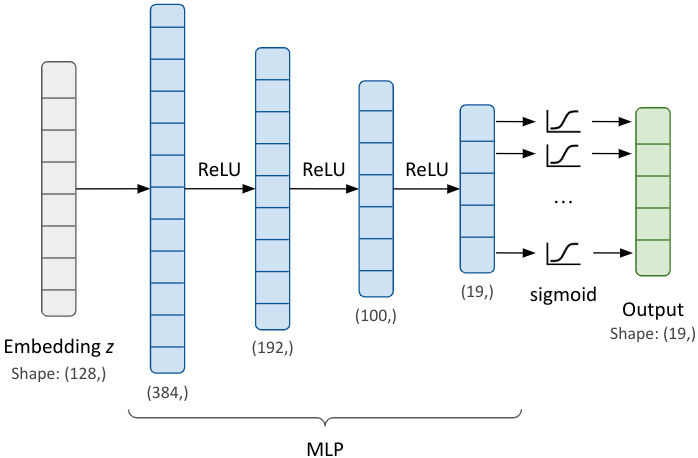
\includegraphics[width=\linewidth]{figures/mlp.png}
   \caption{Multi-label classification with the MLP.}
   \label{fig:mlp}
\end{figure}

While linear probing offers a straightforward approach, its limited approximation capabilities hinder its ability to capture complex relationships between the embeddings and class labels. In this experiment, a multi-layer perceptron (MLP) is used as classifier on top of the foundation model because of its enhanced approximation capabilities. By stacking multiple layers, the MLP can model complex patterns within the data, potentially leading to improved results. \\
The utilized a MLP consists of four layers, as illustrated in Fig. \ref{fig:mlp}. The classifier is trained using cross-entropy loss and the Adam optimizer with a learning rate of 0.001. To enhance performance, the learning rate is reduced when the validation loss stagnates. \\
Table \ref{tab:classification} shows the results in comparison with the linear probing. Further, results of a benchamrk classifier model for the BigEarthNet-S2 dataset with 43 classes are provided. As expected, the MLP classifier achieves significantly better results than linear probing. Among the foundation models, the MoCo-v2 model additionally trained on the geo-location classification pretext task outperforms the others. However, contrastive learning with temporal positive pairs does not lead to a performance increase in comparison with the original MoCo-v2. This pretraining approach is not advantageous for this specific multi-label classification downstream task, although previous work by Ayush et al. \cite{geoAwareSelfSuper} reported performance gains in various other downstream tasks such as image segmentation and object detection. \\
The baseline model - the K-Branch CNN - introduced by Sumbul et al. \cite{benchmark}, is specifically designed for multi-label classification of high-dimensional remote sensing images. It is trained directly on the BigEarthNet-S2 images without using a foundation model. This approach considers the complex spatial and spectral content of image local areas by defining spatial resolution-specific CNN branches followed by a multi-attention strategy to handle the importance scores of different local areas of each image. \\ 
Despite the K-Branch CNN's classification task involving all 43 classes, compared to the simpler 19-label classification of the foundation models, it still outperforms the four examined contrastive learning models.
However, given that the K-Branch CNN is fully optimized for the BigEarthNet-S2 data and the MLP only uses small feature embeddings of size 128, optimized for a different dataset (fMoW), the MLP results are impressive. The foundation models appear to generalize well, retaining the most useful information from the $120\times120$ Sentinel-2 images within an embedding vector of only 128 dimensions.  \\

\subsection{Discussion}

A significant limitation of the current experiments is the absence of complete transfer learning. Transfer learning typically involves fine-tuning the pre-trained model on the specific downstream task. This fine-tuning step was skipped in the experiments due to lack of computational ressources. Introducing a retraining phase for the foundation models' weights with a small learning rate could potentially lead to substantial performance improvements. \\
This shows further that the evaluation results are highly dependent on the adaptation mechanism and amount of optimization used. The performance improved significatly when using an MLP instead of linear probing which makes it difficult to evaluate the quality of a foundation model. This is a common downside of extrinsic evaluation \cite{foundationModels}. \\
The BigEarthNet dataset is large, offering a lot of test data for meaningful evaluation and making it sufficiently robust to train large models like the K-Branch CNN from scratch. This makes it difficult for foundation models to outperform the K-Branch CNN. The power of foundation models is more evident when dealing with smaller datasets, where transfer learning can provide significant better results with less overfitting compared to models trained from scratch.